% !TeX root = ..\main.tex
\npchapter{Performanceanalyse} \label{ch:performanceAnalysis}
In diesem Kapitel wird die Performance von Bun ausführlich untersucht und mit Node.js verglichen. Hierbei liegt der Fokus darauf, die Leitfrage \glqq Welche konkreten Leistungsverbesserungen können in Bun 1.0 im Vergleich zu Node.js festgestellt werden, und wie lassen sie sich quantifizieren?\grqq{} zu beantworten (siehe \autoref{ch:introduction}). Zuerst wird die Vorgehensweise bei den Tests vorgestellt. Anschließend wird der verwendete Versuchsaufbau erläutert. Vor der Betrachtung der Ergebnisse folgt die Vorstellung der Beispielimplementierungen.


\section{Vorgehensweise} \label{sec:performance-approach}
Als Metriken für die Performanceanalyse werden die durchschnittliche Latenz, die Anzahl an HTTP-Anfragen pro Sekunde, der Anteil an erfolgreichen HTTP-Anfragen, die CPU-Auslastung und der maximal genutzte Arbeitsspeicher während der Ausführungszeit verwendet. Denn diese spiegeln die in der Theorie erarbeiteten Charakteristiken wider (siehe \autoref{sec:foundations-Performance}). Um die Metriken zu ermitteln, werden verschiedene Testszenarien mit unterschiedlichen Implementierungen betrachtet (siehe \autoref{sec:performance-implementations}). Diese sind auf variierende APIs der Laufzeitumgebungen zurückzuführen. Dadurch werden die Performance von Bun und Node.js bewertet.\\

\noindent
Zuerst erfolgt die Messung der grundlegenden Performance von HTTP-Servern in beiden Laufzeitumgebungen (siehe \autoref{subsec:httpServer}). Dabei greifen 500 gleichzeitige Benutzer für 30 Sekunden auf den Server zu und erhalten einen kurzen Text als Antwort zurück. Dieses Szenario dient der Untersuchung der grundlegenden Netzwerkgeschwindigkeit beider Laufzeitumgebungen. Als nächstes wird ein Datei-Server verwendet, der jedem Aufrufer ein Bild zurückgibt (siehe \autoref{subsec:fileServer}). Dieser Test wird für 50, 250, 500 und 1.000 gleichzeitige Nutzer über einen Zeitraum von 30 Sekunden durchgeführt. Die Last wird variiert, um die Server näher an ihre Grenzen zu bringen. Der letzte Testfall berechnet die Fibonacci-Folge für die Zahl 45, um die Leistung beider Laufzeitumgebungen bei rechenintensiven Aufgaben zu evaluieren (siehe \autoref{subsec:fibonacci}).

\noindent
Um die Performance korrekt zu bestimmen, müssen geeignete Tools verwendet werden. In dieser Arbeit kommen folgenden Tools zum Einsatz:

\begin{itemize}
	\item Bombardier Version 1.2.6,
	\item GNU Time.
\end{itemize}

\noindent
Bombardier generiert die HTTP-Anfragen an die Server in den ersten beiden Testszenarien. Mit diesem Tool kann die Dauer der Lasttests sowie die Anzahl der zu versendenden Anfragen konfiguriert werden. Außerdem lässt sich festlegen, wie viele gleichzeitige Benutzer simuliert werden. Nach dem Test liefert Bombardier durchschnittliche und maximale Werte für die Anzahl der Anfragen pro Sekunde und die Latenz, einschließlich der Standardabweichung. Zusätzlich schlüsselt das Tool die erhaltenen HTTP-Statuscodes auf. Dadurch kann der Anteil an erfolgreichen und nicht erfolgreichen Anfragen bestimmt werden. Bombardier eignet sich aufgrund seinen detailreichen Aufgaben und seiner Performance. Es ist in Go geschrieben und verwendet das Paket ``fasthttp`` anstelle der nativen HTTP-Implementierung von Go. Dadurch ist es ausreichend performant.\cite{Fedoseev.2016}\newline
Zur Erfassung der CPU-Auslastung und des maximal genutzten Arbeitsspeichers wird GNU Time verwendet. GNU Time ist auf Ubuntu bereits nativ verfügbar und daher gut geeignet \cite{FreeSoftwareFoundation.2018}. Auf MacOS wird eine entsprechende Portierung dieses Tools genutzt, um vergleichbare Daten zu erheben.\newline
Um möglichst repräsentative Ergebnisse zu erzielen, werden alle Testszenarien für jede Laufzeitumgebung jeweils 5-mal wiederholt. Die Durchschnittswerte aus den gesammelten Daten senken die Auswirkung einzelner Abweichungen.


\section{Versuchsaufbau} \label{sec:performance-testSetup}
Um eine konsistente und kontrollierte Umgebung für die Tests zu gewährleisten, werden diese auf spezifischer Hard- und Software durchgeführt. Das Ziel besteht darin, die Testergebnisse reproduzierbar zu gestalten, damit diese unabhängig verifiziert werden können. Aus der Reproduzierbarkeit folgt eine einheitliche Quantifizierung der Ergebnisse zwischen Bun und Node.js. Diese ist notwendig, um die Vergleichbarkeit zu gewährleisten.

\begin{table}[h]
	\caption[Hardware für die Performanceanalyse]{Hardware für die Performanceanalyse\protect\linebreak\textit{Quelle: Eigene Darstellung}}
	\label{table:hardware}
	\centering
	\begin{tabular}{|p{4.5cm}|p{4.5cm}|p{4.5cm}|p{4.5cm}|}
		\hline
		Name & Desktop-PC & MacBook Pro \\
		\hline
		Prozessor & AMD Ryzen 7 2700 @ 3,6 GHz & Apple M1 Pro \\
		\hline
		Arbeitsspeicher & 32 GB DDR4-3200 & 16 GB LPDDR5-6400 \\
		\hline
		Betriebssystem & Ubuntu 23.10 & MacOS 14 Sonoma \\
		\hline
	\end{tabular}
\end{table}

\noindent
\autoref{table:hardware} zeigt die verwendete Hardware und die dazugehörigen Betriebssysteme. Die Verwendung von mehreren Betriebssystemen inklusiver unterschiedlicher Hardware ermöglicht die Verifikation, ob etwaige Performance-Verbesserungen auf eine spezifische Systemumgebung zurückzuführen sind. Die native Implementierung von Bun für Windows ist experimentell und ist für die Öffentlichkeit nicht zugänglich \cite{Verhelst.2023}. Daher ist es nicht möglich, die Funktionsweise von Bun unter Windows zu testen.

\noindent
Die folgenden Versionen der betrachteten Frameworks werden eingesetzt:
\begin{itemize}
	\item Bun Version 1.0.6 (Neuste Version\footnote{Stand 14.10.2023\label{footnote:Stand}})
	\item Node.js Version 18.18.2 (\ac{lts}\footref{footnote:Stand}) \todo{Abkürzung überall verwenden}
	\item Node.js Version 21.0.0 (Neuste\footref{footnote:Stand})
\end{itemize}

\noindent
Die neuste Version von Bun wird für die Tests verwendet, da sie im Vergleich zur Version 1.0 bereits Fehlerkorrekturen enthält \cite{Sumner.2023b}. Bei der Analyse von Node.js werden zwei Versionen einbezogen. Einerseits die Version mit \ac{lts}, da Node.js diese Version für die meisten Benutzer aufgrund des langfristigen Supports empfiehlt \cite{OpenJSFoundation.o.J.}. Andererseits die neuste Version von Node,js, da diese im Vergleich zur \ac{lts}-Version mehrere Verbesserungen für die Performance enthält \cite{OpenJSFoundation.2023b}. Dazu gehört beispielsweise die neuste Version des URL-Parsers Ada. Alleine der aktualisierte URL-Parser verspricht signifikante Performance-Verbesserungen \cite{OpenJSFoundation.2023}.\newline
Der Versuchsaufbau stellt sicher, dass die Performance-Tests auf aussagekräftige und vergleichbare Ergebnisse hinarbeiten und somit der Untersuchung der ersten Forschungsfrage (siehe \autoref{sec:introduction-target}) dienen.

\section{Implementierungen} \label{sec:performance-implementations}
Im Folgenden werden die für jedes Testszenario (siehe \autoref{sec:performance-approach}) verwendeten Implementierungen vorgestellt.

\subsection{HTTP-Server} \label{subsec:httpServer}
Um die grundlegende Performance von Netzwerkanfragen zu bestimmen, werden zwei einfache Programme verwendet. Die Latenz spiegelt die Reaktionszeiten der betrachteten Laufzeitumgebungen wider, da sowohl Client als auch Server auf demselben Endgerät stattfinden und somit keine Verzögerungen durch das Netzwerk auftreten. In \autoref{fig:httpServerBun} ist der Quellcode für Bun dargestellt, während \autoref{fig:httpServerNode} den Quellcode für Node.js zeigt.

\begin{lstlisting}[caption={[HTTP-Server Bun]HTTP-Server Bun\\\textit{Quelle: Eigene Darstellung}},label={fig:httpServerBun}]
	Bun.serve({
		port: 3000,
		fetch(request) {
			return new Response("Hello from Bun!");
		},
	});
\end{lstlisting}

\begin{lstlisting}[caption={[HTTP-Server Node.js]HTTP-Server Node.js\\\textit{Quelle: Eigene Darstellung}},label={fig:httpServerNode}]
	import http from "node:http";
	
	http.createServer(function (request, response) {
		response.write('Hello from Node.js!')
		response.end();
	}).listen(3000);
\end{lstlisting}

\noindent
Um die Performance dieser Programme zu testen, werden mit Bombardier 500 gleichzeitige Benutzer für eine Dauer von 30 Sekunden simuliert, wie im Befehl in \autoref{fig:bombardierHttpServer} visualisiert.

\begin{lstlisting}[caption={[Bombardier HTTP-Server]Bombardier HTTP-Server\\\textit{Quelle: Eigene Darstellung}},label={fig:bombardierHttpServer}]
	bombardier -c 500 -d 30s http://localhost:3000
\end{lstlisting}

\noindent
Die Server werden mit der jeweiligen Laufzeitumgebung gestartet. Zur Ermittlung der CPU- und RAM-Auslastung wird GNU Time verwendet. Die Befehle zur Messung der CPU- und RAM-Auslastung sind in Ubuntu und MacOS in den Abbildungen \ref{fig:timeHTTPServerUbuntu} und \ref{fig:timeHTTPServerMacOS} dargestellt. Um dieselben Messungen mit Node.js durchzuführen, muss \textit{bun} durch \textit{node} ersetzt werden.

\begin{lstlisting}[caption={[CPU- und RAM-Messung auf Ubuntu]CPU- und RAM-Messung auf Ubuntu\\\textit{Quelle: Eigene Darstellung}},label={fig:timeHTTPServerUbuntu}]
	/usr/bin/time -f "Execution Time: %e\nMaximum Resident Set Size (RSS): %M\nPercent of CPU This Job Got: %P" bun httpServer.js
\end{lstlisting}

\begin{lstlisting}[caption={[CPU- und RAM-Messung auf macOS]CPU- und RAM-Messung auf macOS\\\textit{Quelle: Eigene Darstellung}},label={fig:timeHTTPServerMacOS}]
	gtime -f "Execution Time: %e\nMaximum Resident Set Size (RSS): %M\nPercent of CPU This Job Got: %P" bun httpServer.js
\end{lstlisting}

\todo{Beispiel-Ausgabe von Bombardier zeigen, um zu erklären, welche Daten pro Testdurchlauf erfasst werden}

\subsection{Datei-Server} \label{subsec:fileServer}
Im zweiten Szenario wird die Abfrage von Bilddateien simuliert. Denn ein Bild stellt eine große Datenmenge da und prüft so den Austausch großer Datenmengen. Dieser Prozess inkludiert die Performance von Zugriffen auf das Dateisystem. Die Implementierungen für Bun und Node.js sind in den Abbildungen \ref{fig:fileServerBun} und \ref{fig:fileServerNode} dargestellt.

\begin{lstlisting}[caption={[Datei-Server Bun]Datei-Server Bun\\\textit{Quelle: Eigene Darstellung}},label={fig:fileServerBun}]
	const basePath = "../data";
	
	Bun.serve({
		port: 3000,
		fetch(request) {
			const filePath = `${basePath}${new URL(request.url).pathname}`;
			
			try {
				return new Response(Bun.file(filePath));
			} catch (error) {
				return new Response("File not found", {
					status: 404
				});
			}
		},
	});
\end{lstlisting}

\begin{lstlisting}[caption={[Datei-Server Node.js]Datei-Server Node.js\\\textit{Quelle: Eigene Darstellung}},label={fig:fileServerNode}]
	import { createReadStream } from "node:fs";
	import http from "node:http";
	
	const basePath = "../data";
	
	http.createServer((request, response) => {
		const filePath = `${basePath}${request.url}`;
		const readStream = createReadStream(filePath);
		
		readStream.on("open", () => {
			response.setHeader("content-type", "image/png");
			response.writeHead(200);
			
			readStream.pipe(response);
		});
		
		readStream.on("error", () => {
			response.writeHead(404, "Image not found");
			response.end();
		});
	}).listen(3000);
\end{lstlisting}

\noindent
Beide Server rufen dasselbe Bild aus dem Dateisystem ab, da in jeder Anfrage derselbe Pfad angegeben wird. Falls unter dem angeforderten Pfad keine Datei gefunden wird, geben beide Server eine entsprechende Fehlermeldung zurück. Dieses Testszenario wird jeweils mit 50, 250, 500 und 1.000 gleichzeitigen Benutzern für eine Dauer von 30 Sekunden getestet (siehe \autoref{sec:performance-approach}). Der Befehl für 50 gleichzeitige Benutzer ist in \autoref{fig:bombardierFileServer} dargestellt. Die Befehle zur Messung der CPU- und RAM-Auslastung unterscheiden sich nicht im Vergleich zum HTTP-Server (siehe \autoref{subsec:httpServer}).

\begin{lstlisting}[caption={[Bombardier Datei-Server]Bombardier Datei-Server\\\textit{Quelle: Eigene Darstellung}},label={fig:bombardierFileServer}]
	bombardier -c 500 -d 30s http://localhost:3000/example.png
\end{lstlisting}

\subsection{Berechnung der Fibonacci-Folge} \label{subsec:fibonacci}
Als letztes Szenario wird die Fibonacci-Folge für die Zahl 45 berechnet, um die Leistung bei der Ausführung rechenintensiver Aufgaben zu bewerten. Hierfür nutzen beide Laufzeitumgebungen die in \autoref{fig:fibonacci} dargestellte Implementierung.

\begin{lstlisting}[caption={[Berechnung der Fibonacci-Folge]Berechnung der Fibonacci-Folge\\\textit{Quelle: Eigene Darstellung}},label={fig:fibonacci}]
	const fibonacci = (number) => {
		if (number <= 0) {
			return 0;
		} else if (number <= 1) {
			return 1;
		} else if (number <= 2) {
			return 2;
		}
		
		return fibonacci(number-1) + fibonacci(number-2);
	};
	
	console.log(fibonacci(45));
\end{lstlisting}

\noindent
Das Programm wird mit beiden Laufzeitumgebungen und GNU Time zur Erhebung der notwendigen Metriken ausgeführt. \autoref{fig:timefibonacciUbuntu} stellt dies beispielsweise für Node.js unter Ubuntu dar. Auf MacOS muss \textit{/usr/bin/time} durch \textit{gtime} ersetzt werden.
\begin{lstlisting}[caption={[Messung der Fibonacci-Folge auf Ubuntu]Messung der Fibonacci-Folge auf Ubuntu\\\textit{Quelle: Eigene Darstellung}},label={fig:timefibonacciUbuntu}]
	/usr/bin/time -f "Execution Time: %e\nMaximum Resident Set Size (RSS): %M\nPercent of CPU This Job Got: %P" node fibonacci.js
\end{lstlisting}



\section{Ergebnisse} \label{sec:performance-results}
Im Folgenden werden die Ergebnisse der Testszenarien vorgestellt. Im Anschluss folgt die Diskussion über die daraus resultierenden Vor- und Nachteile.\\

\noindent
\textbf{HTTP-Server Performance}
\begin{figure}[h!]
	\centering
	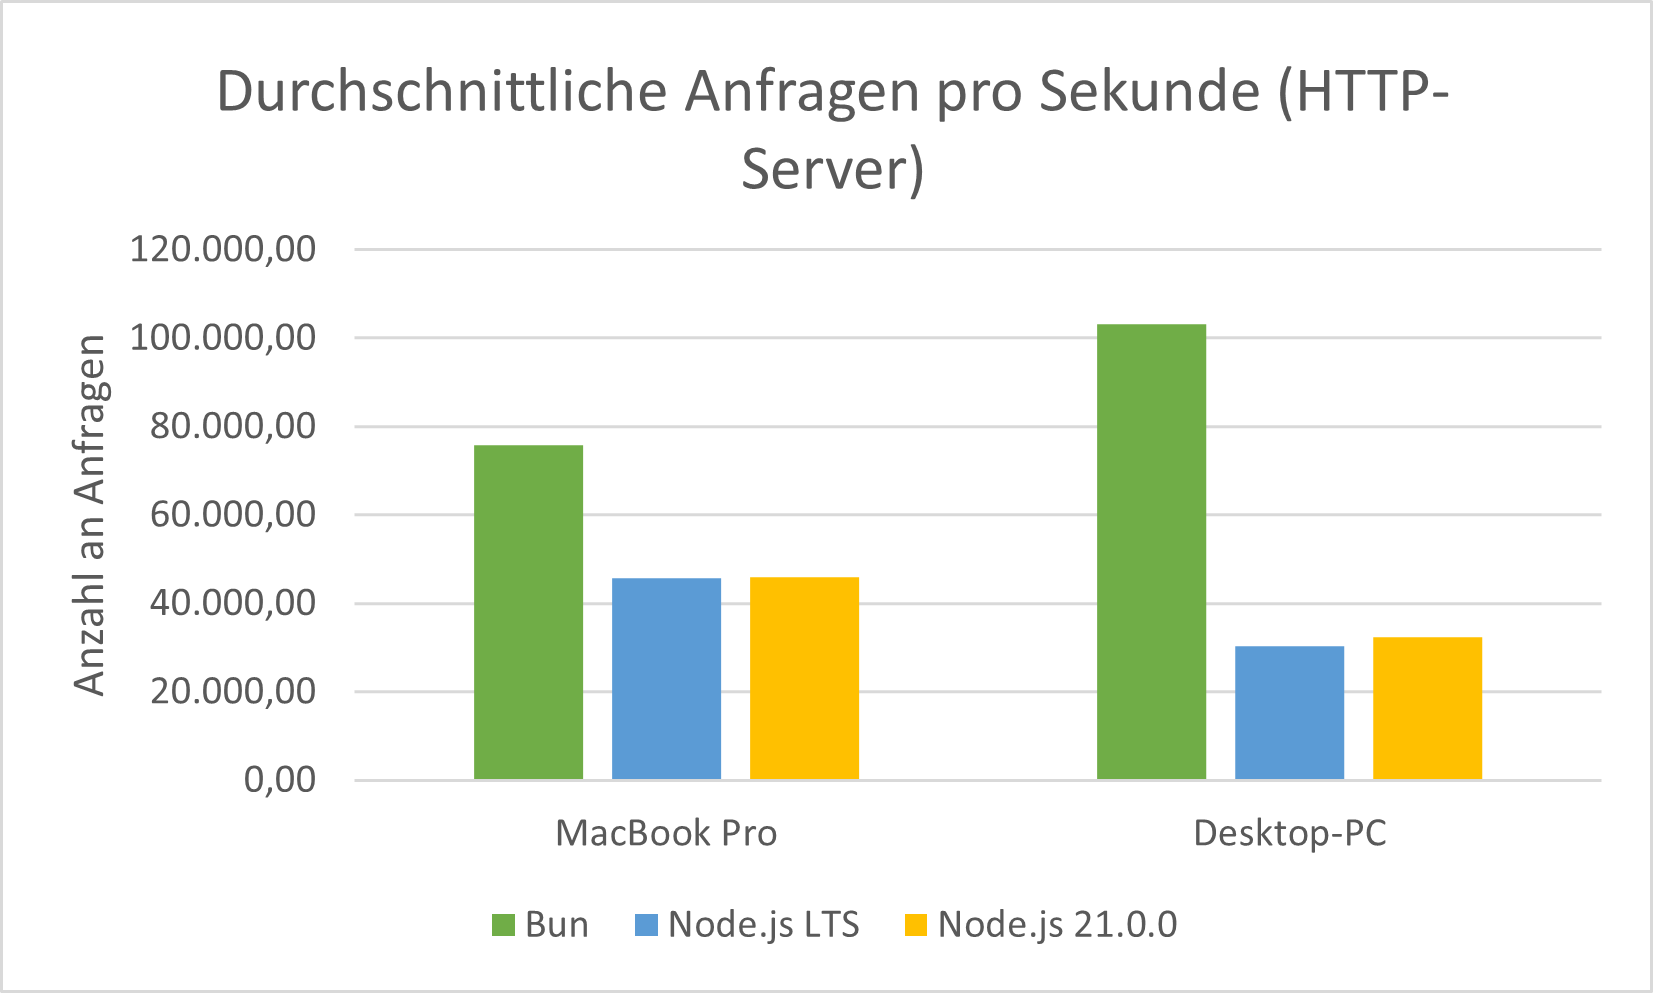
\includegraphics[width=\linewidth]{./images/httpServerAverageRequestsPerSecond.png}
	\caption{HTTP-Server - Durchschnittliche Anzahl an Anfragen pro Sekunde}
	\label{fig:httpServerAverageRequestsPerSecond}
	\textit{Quelle: Eigene Darstellung}
\end{figure}


\noindent
Im ersten Testszenario wurde die grundlegende Leistung der HTTP-Server verglichen. \autoref{fig:httpServerAverageRequestsPerSecond} zeigt die durchschnittliche Anzahl an Anfragen pro Sekunde, die jede Laufzeitumgebung bewältigen konnte. Bun übertraf auf beiden getesteten Geräten sowohl die LTS-Version als auch die neueste Version von Node.js. Bun konnte auf dem Desktop-PC pro Sekunde ungefähr 103.000 Anfragen bewältigen, während Node.js LTS und die neueste Version nur 30.000 bzw. 32.000 Anfragen pro Sekunde verarbeiten konnten. Diese Leistungsunterschiede spiegelten sich auch in den Latenzzeiten wider. Bun hatte eine Latenz von 6,61ms auf dem MacBook Pro und 4,84ms auf dem Desktop-PC, verglichen mit ungefähr 10 ms (MacBook Pro) und etwa 16 ms (Desktop-PC) für Node.js (siehe auch \autoref{fig:httpServerAverageLatency} in \autoref{sec:benchmark-results-diagrams}).\newline
Diese signifikanten Unterschiede deuten darauf hin, dass Bun das Potential bietet, in realen Szenarien erheblich schneller zu sein als Node.js. Diese Erkenntnisse legen nahe, dass die Verwendung der JavaScriptCore Engine und der Programmiersprache Zig klare Vorteile bei der Bewältigung von Netzwerkanfragen bietet. Das hat erhebliche Auswirkungen auf die Effizienz und Skalierbarkeit in Produktionsumgebungen.\\

\noindent
\textbf{Datei-Server Performance}
\begin{figure}[h!]
	\centering
	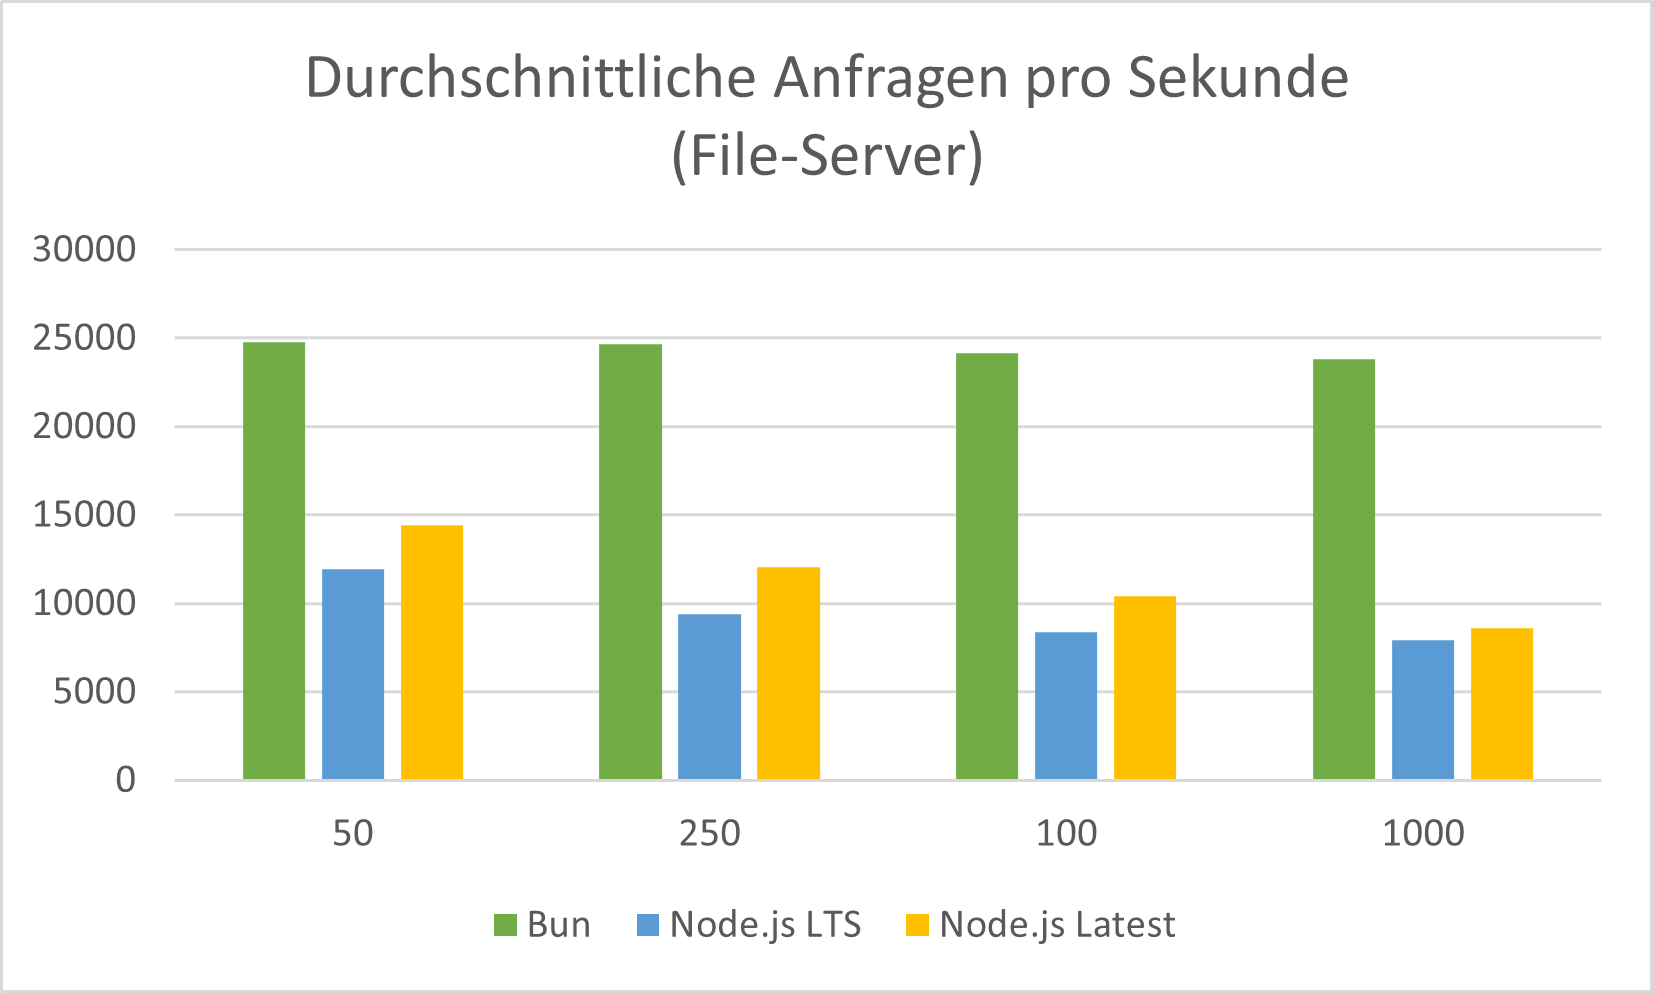
\includegraphics[width=\linewidth]{./images/fileServerAverageLatencyDesktop.png}
	\caption{Datei-Server - Durchschnittliche Latenz}
	\label{fig:fileServerAverageLatency}
	\textit{Quelle: Eigene Darstellung}
\end{figure}

\noindent
Das zweite Testszenario analysiert, inwiefern die Potentiale aus dem ersten Test in einem realen Anwendungsfall umgesetzt werden. Um die Diagramme übersichtlich zu halten, konzentriert sich die Darstellung auf den Desktop-PC. Denn die Unterschiede und Trends sind auf beiden Geräten ähnlich. \autoref{fig:fileServerAverageLatency} zeigt die durchschnittlichen Latenzen beim Zugriff auf Bilddateien. Bun schnitt erneut besser ab als Node.js. Bei 50 gleichzeitigen Benutzern betrug die Latenzzeit für Bun 2 ms, während Node.js LTS und die neueste Version Latenzen von 4,2 ms bzw. 3,5 ms aufwiesen. Diese Unterschiede wurden bei steigender Anzahl gleichzeitiger Benutzer noch deutlicher. Bei 250 Nutzern beläuft sich Buns Latenz auf ca. 10ms, der beste Wert von Node.js liegt bei ca. 21ms (Neuste Version). Bei 1.000 gleichzeitigen Benutzern benötigte Bun durchschnittlich 42 ms für die Antwort, während Node.js bei 116 ms (neueste Version) lag. Die Unterschiede von mehr als 50\% führen zu erheblich schnelleren Ladezeiten von Webseiten, insbesondere bei einer hohen Anzahl von Bildern. Dadurch, dass Bun die Anfragen selbst deutlich schneller beantwortet, bewältigt Bun gleichzeitig deutlich mehr Anfragen pro Sekunde. Trotz der höheren Effizienz konnte Bun alle Anfragen erfolgreich beantworten, unabhängig von der Anzahl gleichzeitiger Benutzer. In der neuesten Version von Node.js wurden ab 250 gleichzeitigen Benutzern nicht mehr alle Anfragen erfolgreich beantwortet. Bei 1.000 gleichzeitigen Nutzern sank die Erfolgsrate auf dem MacBook Pro auf 99,54\%. Bun erzielte bei 50, 250 und 500 gleichzeitigen Benutzern eine hundertprozentige Erfolgsrate bei der Beantwortung aller Anfragen. Bei 1.000 simulierten Anwendern sank die Erfolgsrate auf 99,96\%. Node.js LTS zeigte ebenfalls eine sehr hohe Erfolgsrate, bei der erst ab 1.000 gleichzeitigen Benutzern fehlerhafte Antworten zurückgeliefert wurden, was zu einer Erfolgsrate von 99,92\% führte. Obwohl die absolute Anzahl der Anfragen mit Fehlern sehr niedrig war, ist es dennoch bemerkenswert, dass die neueste Version von Node.js hier deutlich größere Defizite aufwies. Möglicherweise sind Fehler im neusten Release enthalten, die diese Leistungsunterschiede erklären.\\

\begin{figure}[h!]
	\centering
	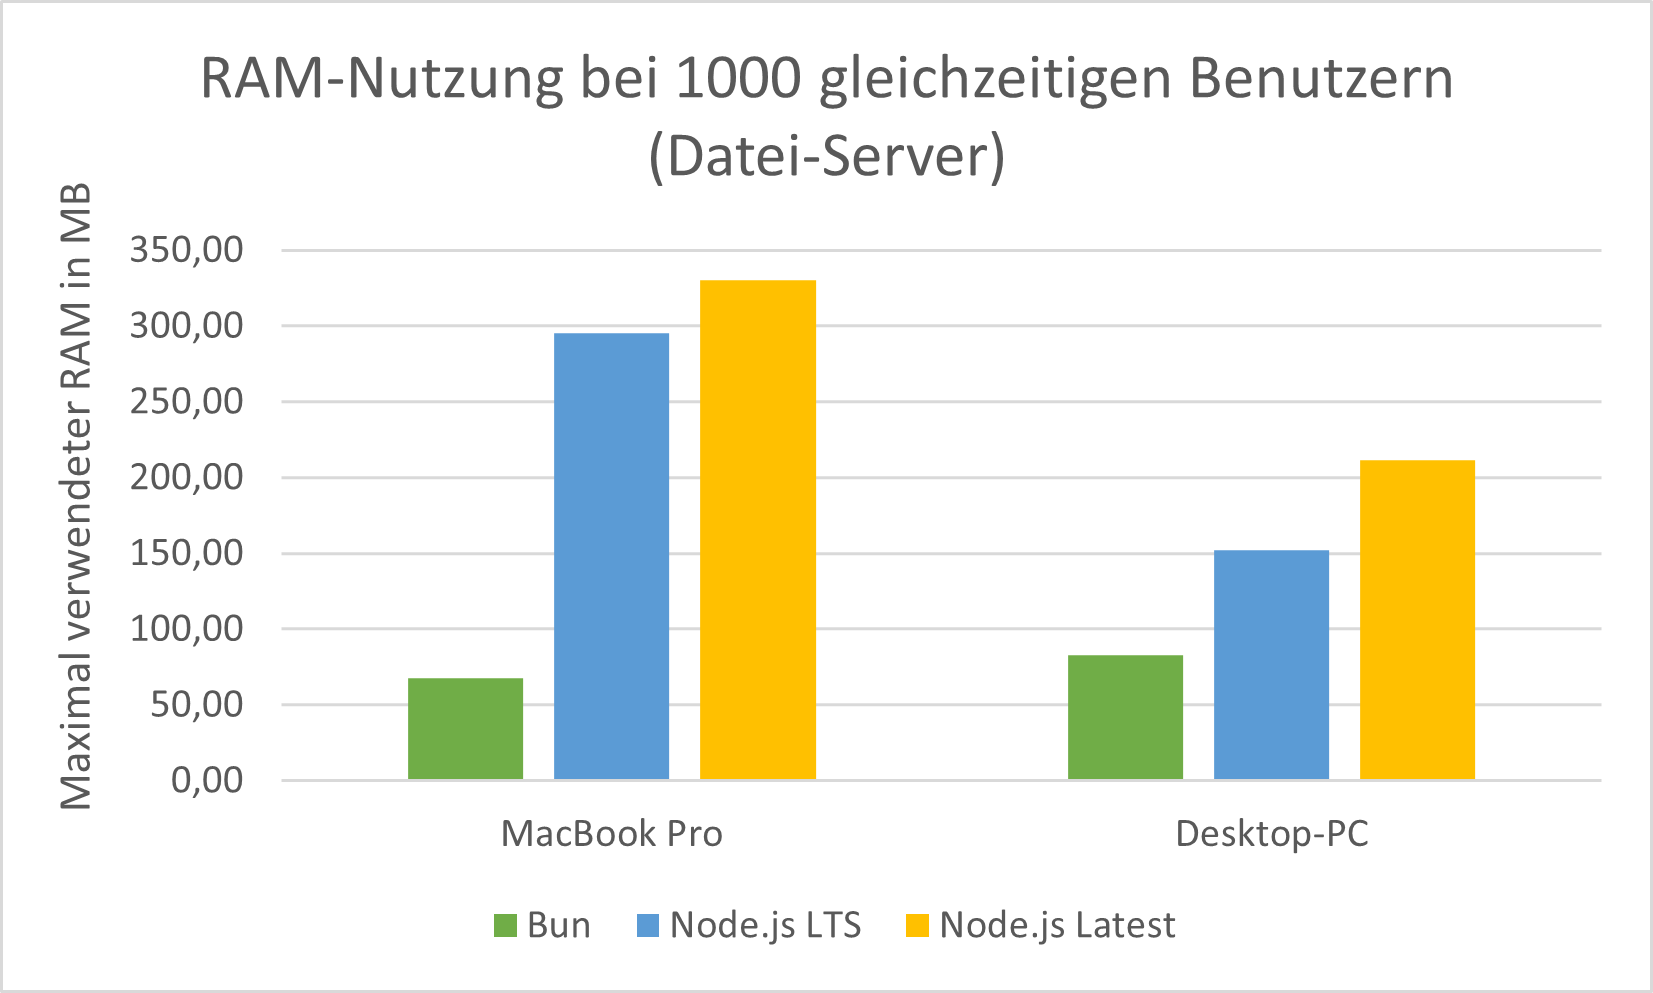
\includegraphics[width=\linewidth]{./images/fileServerRamUsage.png}
	\caption{Datei-Server - Maximal verwendeter Arbeitsspeicher}
	\label{fig:fileServerRamUsage}
	\textit{Quelle: Eigene Darstellung}
\end{figure}


\noindent
Die RAM- und CPU-Nutzung der Laufzeitumgebungen werden bei 1.000 gleichzeitigen Benutzern verglichen. Denn bei der höchsten Last sind die Differenzen am besten zu erkennen. \autoref{fig:fileServerRamUsage} zeigt den maximal verwendeten Arbeitsspeicher während des 30-sekündigen Tests. Bun war auch hier effizienter als Node.js auf beiden getesteten Geräten. Auf dem MacBook Pro verbrauchte Bun etwa 56 MB Arbeitsspeicher, während Node.js LTS und die neueste Version etwa 296 MB bzw. 330 MB benötigten. Auf dem Desktop-PC betrug der Arbeitsspeicherverbrauch von Bun etwa 84 MB, im Vergleich zu 152 MB (LTS) bzw. 212 MB (neueste Version) bei Node.js. Die Beobachtungen deuten auf klare Vorteile in Bezug auf Effizienz und Kosten hin. Bun kann mit begrenzten Ressourcen anspruchsvollere Aufgaben bewältigen.\\

\begin{figure}[h!]
	\centering
	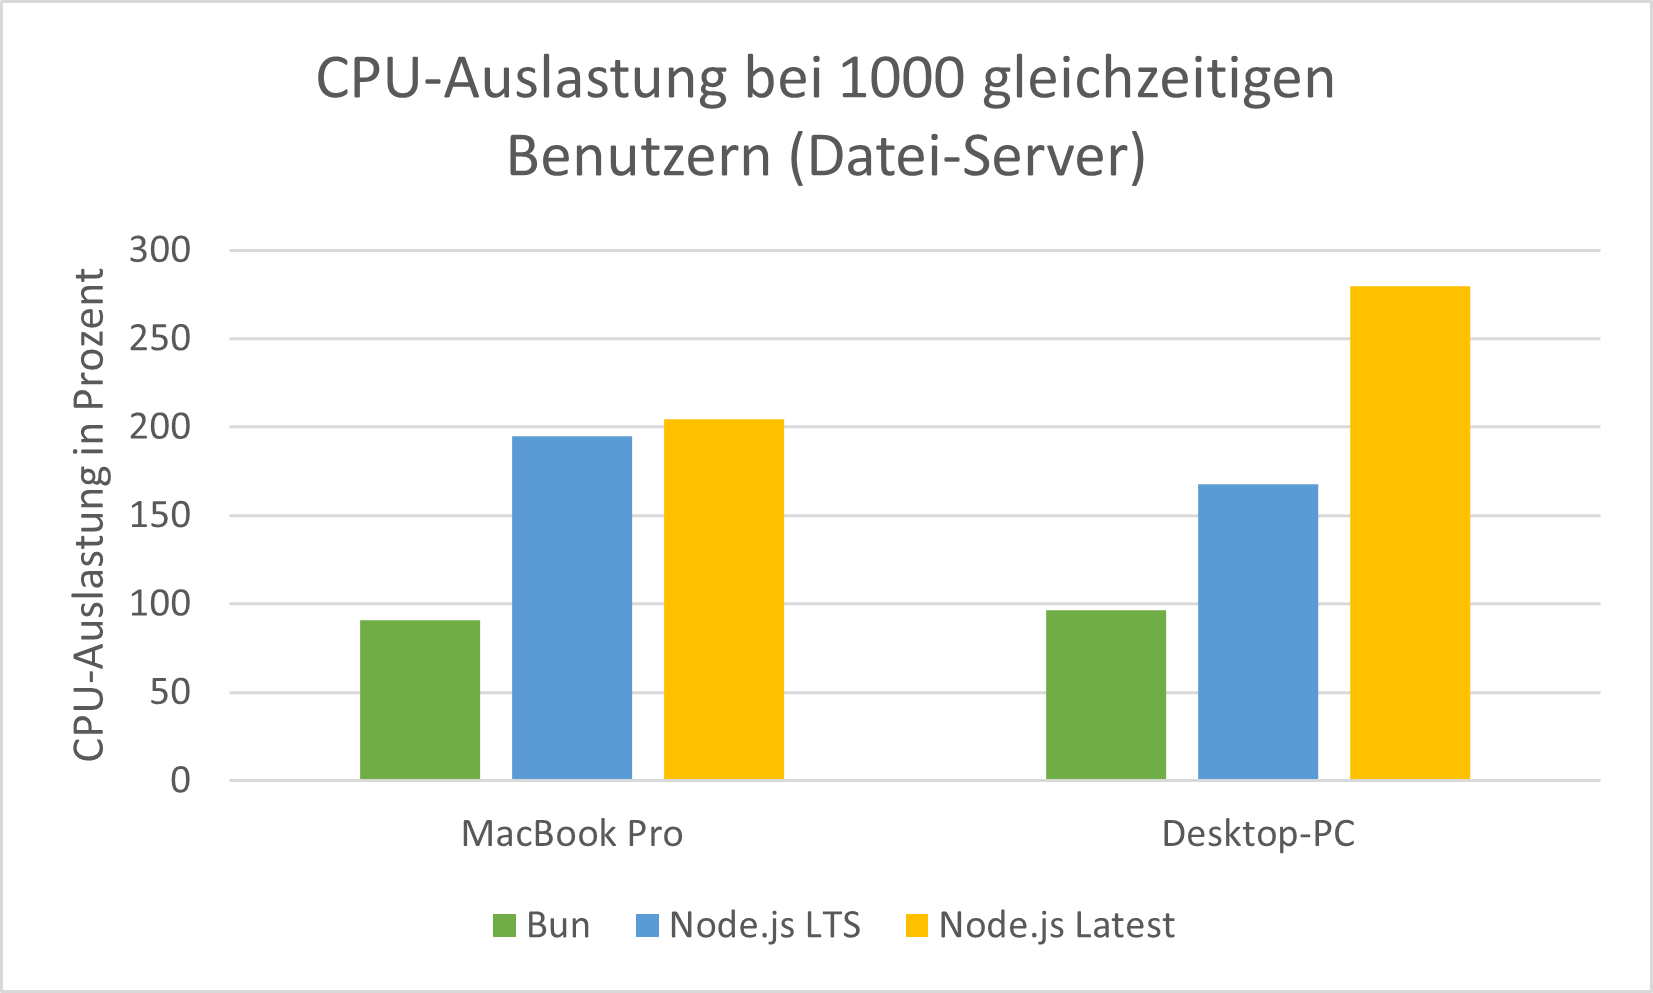
\includegraphics[width=\linewidth]{./images/fileServerCpuUsage.png}
	\caption{Datei-Server - CPU-Auslastung }
	\label{fig:fileServerCpuUsage}
	\textit{Quelle: Eigene Darstellung}
\end{figure}

\noindent
\autoref{fig:fileServerCpuUsage} zeigt die CPU-Auslastung bei 1.000 gleichzeitigen Benutzern in Prozent. Bei der CPU-Auslastung bedeuten 100\%, dass ein Kern vollständig ausgelastet ist. Wenn ein Computer eine CPU mit 4 Kernen besitzt, beträgt die maximale CPU-Auslastung 400\%. Die CPU-Auslastung bestätigt, dass Bun mit den verfügbaren Ressourcen effizienter umgeht als Node.js. Die CPU-Nutzung bei Bun betrug etwa 91\% auf dem MacBook Pro und 96\% auf dem Desktop-PC. Node.js LTS hingegen benötigte etwa 195\% auf dem MacBook Pro und 167\% auf dem Desktop-PC, während die neueste Version noch schlechter abschnitt. Bun kommt mit einem Kern der CPU aus, während Node.js 2 oder auch 3 Kerne beansprucht. D. h. Node.js stellt ungefähr doppelt so starke Anforderungen an die CPU. Diese deutlichen Unterschiede in der CPU-Auslastung und Arbeitsspeichernutzung zeigen, dass Bun bei gleichzeitiger Last effizienter war und anspruchsvolle Aufgaben bewältigen konnte.\\

\noindent
\textbf{Performance bei der Berechnung der Fibonacci-Folge}
\begin{figure}[h!]
	\centering
	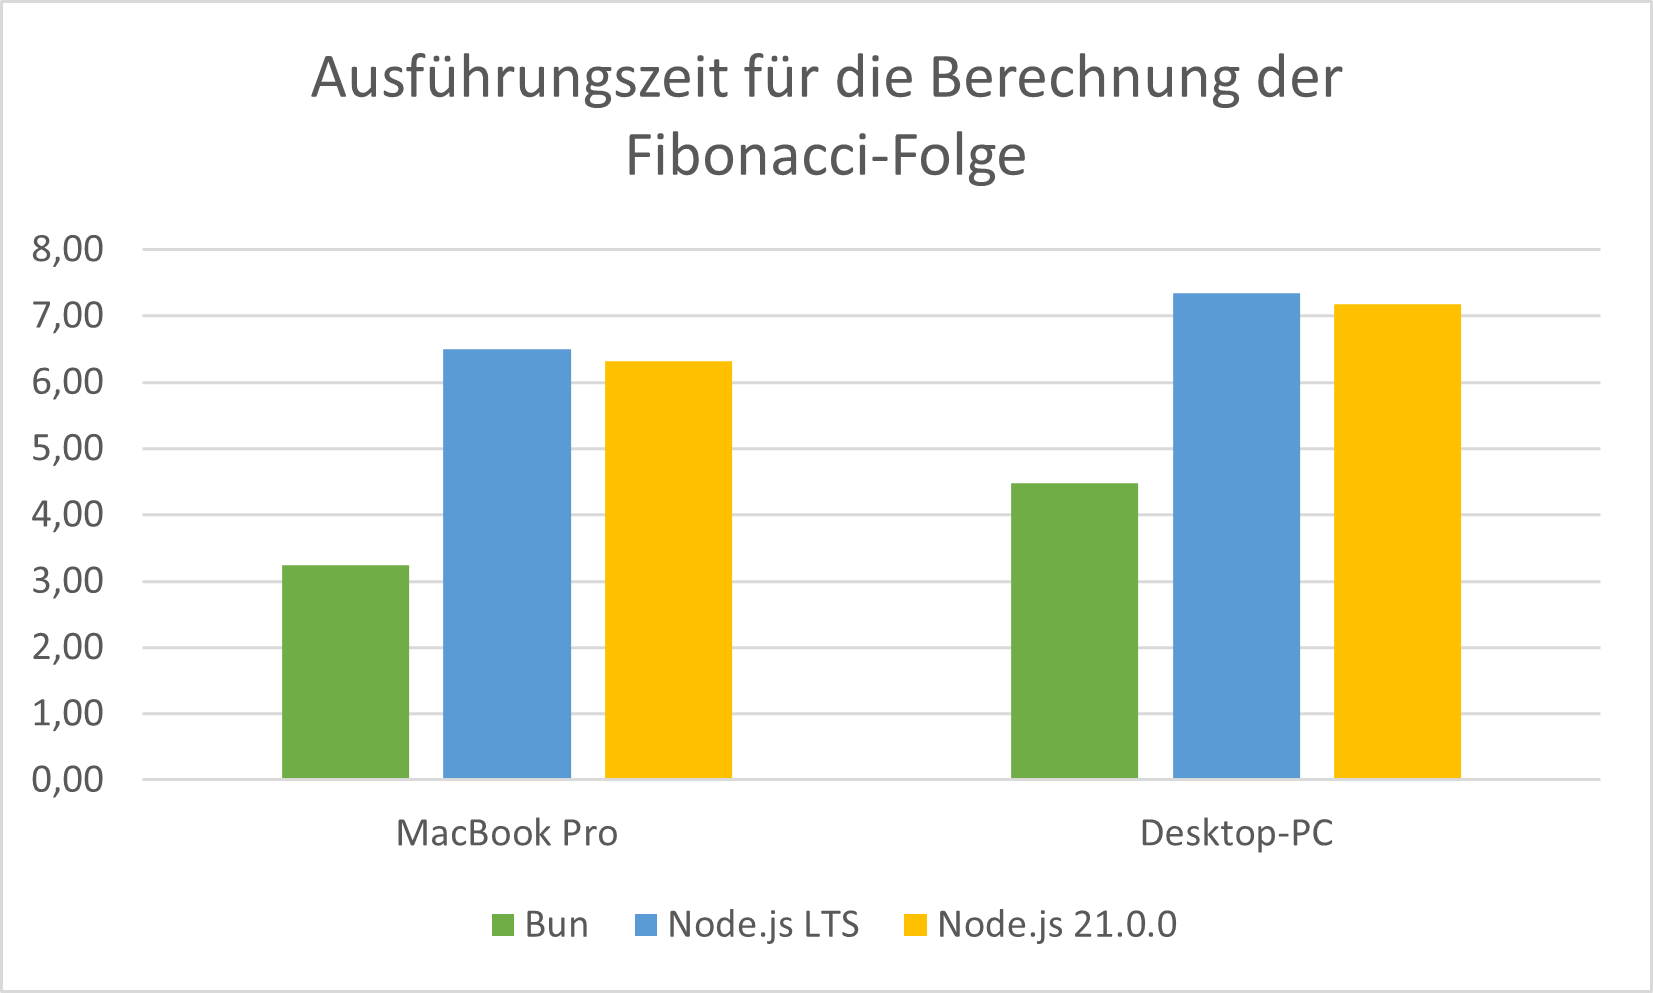
\includegraphics[width=\linewidth]{./images/fibonacciRuntime.png}
	\caption{Ausführungszeit für die Berechnung der Fibonacci-Folge}
	\label{fig:fibonacciRuntime}
	\textit{Quelle: Eigene Darstellung}
\end{figure}


\noindent
Der dritte Testfall konzentriert sich auf die Leistung von Bun und Node.js bei der Ausübung rechenintensiver Aufgaben. Die Ausführungszeiten sind in \autoref{fig:fibonacciRuntime} dargestellt. Bun war erheblich schneller, wobei die Berechnung in durchschnittlich 3,24 Sekunden auf dem MacBook Pro und 4,47 Sekunden auf dem Desktop-PC abgeschlossen wurde. Node.js zeigte kaum Unterschiede zwischen der LTS- und der neuesten Version, wobei die schnellste Berechnung 6,32 Sekunden (MacBook Pro) und 7,18 Sekunden (Desktop-PC) dauerte. Somit ist Bun auf dem MacBook Pro ca. 50\% und auf dem Desktop-PC ungefähr 40\% schneller. Die CPU-Auslastung beträgt sowohl bei Bun als auch bei Node.js ca. 100\%. Der maximal verwendete Arbeitsspeicher unterscheidet sich auf dem Desktop-PC nur um maximal 3 MB. Erwähnenswert ist, dass hier die neuste Version von Node.js 1 MB weniger Arbeitsspeicher als Bun genutzt hat. Auf dem MacBook Pro sind die Unterschiede deutlich größer. Bun benötigt maximal ca. 26 MB RAM, Node.js im Vergleich dazu 42 MB (LTS) und 37 MB (Neuste Version).\newline
Die Betrachtung der CPU-Auslastung, der RAM-Nutzung und der Ausführungszeiten bestätigt die beobachteten Leistungsunterschiede aus den beiden vorherigen Testszenarien. Unabhängig von der betrachteten Metrik weist Bun eine deutlich höhere Leistungsfähigkeit auf beiden Endgeräten auf.

\section{Fazit} \label{sec:performance-conclusion}
Dieses Kapitel widmet sich auf die Beantwortung der ersten Leitfrage \glqq Welche konkreten Leistungsverbesserungen können in Bun 1.0 im Vergleich zu Node.js festgestellt werden, und wie lassen sie sich quantifizieren?\grqq{} (siehe \autoref{ch:introduction}). Die Ergebnisse des Benchmarks verdeutlichen, dass Bun in sämtlichen Testszenarien signifikant bessere Leistungen als Node.js erzielt hat. Dies zeigt sich in einer deutlich reduzierten Latenz, in einer geringeren Inanspruchnahme von Arbeitsspeicher und CPU-Ressourcen während der Verarbeitung von Netzwerkanfragen. Diese Resultate bestätigen sich bei der Ausführung rechenintensiver Aufgaben. Bun hat die Fibonacci-Folge bis zu 50\% schneller berechnet als Node.js. In diesem Szenario beansprucht Bun ähnlich viel Arbeitsspeicher wie Node.js, weist jedoch eine geringere CPU-Auslastung auf. \newline
Die Ergebnisse unterstreichen, dass Bun im Entwicklungsprozess gute Entscheidungen bei der Auswahl seiner Komponenten getroffen hat. Die JavaScriptCore Engine nutzt ihre mehreren \ac{jit-compiler} (siehe \autoref{sec:foundations-Bun}) für eine effizientere Optimierung des Maschinencodes. Die Auswahl von Zig als systemnahe Programmiersprache und das intensive Testen während der Entwicklung haben (siehe \autoref{sec:foundations-Bun}) die Effizienz von Bun im Umgang mit den verfügbaren Ressourcen gesteigert.\\

\noindent
Das Benchmark basiert auf den Vergleich ausgewählter Eigenschaften auf einem spezifischen Hardware-Setup. Es ist zu beachten, dass diese Ergebnisse unter Verwendung von Servern aus der Produktionsumgebung potenziell abweichen können. Die Analysen beschränken sich auf einfache Beispiele, die sich auf die Performance der Laufzeitumgebungen konzentrieren. In der Realität sind Anwendungsquellcodes oft umfangreicher und komplexer. Die vorliegenden Ergebnisse geben daher nicht zwangsläufig die Performance solcher Anwendungen wieder. Für eine umfassende Bewertung der Laufzeitleistung sollten die Unterschiede zwischen dem MacBook Pro und dem Desktop-PC genauer analysiert werden. Es ist wichtig, die Gründe für die signifikanten Unterschiede im Anteil erfolgreicher Anfragen zu ermitteln. Die Untersuchung sollte auf andere Hardware-Setups ausgeweitet werden, um die Generalisierbarkeit der Ergebnisse sicherzustellen.